\documentclass[11pt]{article}
\usepackage{amsmath}
\usepackage{amssymb}
\usepackage{graphicx}
\usepackage{geometry}[0.9in]
\usepackage{url}

\renewcommand{\vec}[1]{\boldsymbol{#1}}
\newcommand{\hvec}[1]{\hat{\vec{#1}}}

\title{Clarifications on scattering factors and scattering densities.}
\author{Richard Kirian}
\date{\today}
\begin{document} 

\maketitle

\section{Objective}

We sometimes wish to construct a scattering density for an ensemble of atoms so that we may use a fast Fourier transform method to generate scattering amplitudes.  However, it is usually the atomic form factors and dispersion corrections that are found in the literature (because this is what can be measured).  Here we aim to clarify how to use published tabulations in order to generate our desired scattering density maps.

\section{Atomic scattering density and atomic scattering factor}

Assuming monochromatic plane-wave illumination, far-field x-ray diffraction intensities under the first Born approximation are equal to 
\begin{align}\label{eqn:qrf}
I(\vec{q}) = J_0 \Delta \Omega r_e^2 P(\hvec{k}_\text{in}, \hvec{k}_\text{out}) \left| \sum_n^N f_n(q) \exp(-i \vec{q}\cdot\vec{r}_n)\right|^2
\end{align}
where $J_0$ is the incident photon fluence (photons per area), $\Delta \Omega$ is the solid angle of the detector pixel (assumed to be small), $r_e$ is the classical electron radius, $P(\hvec{k}_\text{in}, \hvec{k}_\text{out})$ is the polarization factor that depends on the incident wavevector direction $\hvec{k}_\text{in}$, and the outgoing wavevector $\vec{k}_\text{out}$, $f_n(q)$ is the atomic scattering factor (assumed rotationally symmetric), $\vec{r}_n$ is the position vector of the $n$th atom, and the wavevector transfer is $\vec{q} = \vec{k}_\text{out}-\vec{k}_\text{in}$.  We may define a continuum of complex \emph{scattering density} $\rho(\vec{r})$ such that
\begin{align}\label{eqn:dft}
I(\vec{q}) = J_0 \Delta \Omega r_e^2 P(\hvec{k}_\text{in}, \hvec{k}_\text{out}) \left| \iiint_{-\infty}^\infty \rho(\vec{r}) \exp(-i \vec{q}\cdot\vec{r}) \; d^3r\right|^2 \; .
\end{align}

If we consider just a single rotationally symmetric atom situated at the origin, the atomic form factor is equal to\footnote{See appendix \ref{sec:3d1d}.}
\begin{align}
f(q)  &= \iiint_{-\infty}^\infty \rho(r) \exp(-i \vec{q}\cdot\vec{r}) \; d^3r \\
  &= \int_0^\infty \rho(r)   \frac{\sin(qr)}{qr}  4\pi r^2 dr \; . \label{eqn:form}
\end{align}
For an atom located at the position $\vec{r}_n$ we have
\begin{align}
f(\vec{q})  = \iiint_{-\infty}^\infty \rho(|\vec{r}-\vec{r}_0|) \exp(-i \vec{q}\cdot\vec{r}) d^3r = f(q)\exp(i \vec{q}\cdot\vec{r}_n)  \; .
\end{align}
We may take the inverse Fourier transforms to arrive at %the expression for the scattering density in terms of the atomic scattering factor:
\begin{align}
\rho(r)  &= \frac{1}{8\pi^{3}} \int  f(q)  \exp(i \vec{q}\cdot\vec{r}) \; d^3q \\
&= \frac{1}{8\pi^{3}} \int_0^\infty f(q)   \frac{\sin(qr)}{qr}  4\pi q^2 dq \; . \label{rhor}
\end{align}
If we are well above resonances, $\rho(\vec{r})$ is well approximated as the electron number density.    Atomic scattering factors are often approximated by a $q$-dependent ``atomic form factor'' $f_0(q)$  that is related to the Fourier transform of the electron density, along with a complex energy-dependent (but $q$-independent) ``anomalous dispersion correction'' $\Delta f(E) =  f'(E) + i f''(E)$: 
\begin{align}
f(q) = f_0(q) + \Delta f(E) \; . %= f_0(q) + f'(E) + i f''(E)  \;.
\end{align}
Plugging these in we have
\begin{align}
\rho(r)  &= \frac{1}{8\pi^{3}} \iiint_{-\infty}^\infty  (f_0(q) + \Delta f(E))   \exp(i \vec{q}\cdot\vec{r}) \; d^3q \\
&=  \delta(\vec{r}) \Delta f(E) + \frac{1}{8\pi^{3}} \int_0^\infty f_0(q)    \frac{\sin(qr)}{qr}  4\pi q^2 dq  \\
&=  \delta(\vec{r}) \Delta f(E) + \rho_0(r) \; .
\end{align}
For an atom at position $\vec{r}_n$ we have
\begin{align}
\rho_n(\vec{r})  &=  \delta(\vec{r}-\vec{r}_n) \Delta f_n(E) + \rho_{0n}(|\vec{r}-\vec{r}_n|) \; .
\end{align}
In order to build our complete scattering density we take the sum
\begin{align}
\rho(\vec{r})  &= \sum_n \delta(\vec{r}-\vec{r}_n) \Delta f_n(E) + \rho_{0n}(|\vec{r}-\vec{r}_n|) \; .
\end{align}
Our chores are to (1) figure out a way to programmatically access the needed scattering factors in order to build a scattering density sampled about a 3D grid, (2) decide on how to lay out delta functions in the typical situation in which the atoms do not lie exactly on grid points, (3) do the transforms in equation \ref{rhor} numerically and perhaps tabulate the results, and (4) efficiently place the resulting $\rho(\vec{r})$ densities into a 3D grid.  As an alternative to step (3) we may look up the electron densities $\rho(r)$ from tabulated calculations.


\section{Hubbel form factors}

Hubbel {\itshape et al.} (1975)\cite{hubbellAtomicFormFactors1975} have provided tables of atomic form factors that are still in widespread use today.  They provide atomic form factors $F(q,Z)$ (atomic number $Z$) that are defined exactly as in equation \ref{eqn:form}.
The form factors $F(q,Z)$ are accessible programatically from the  \texttt{xraylib} library, which has a Python wrapper.

\section{Electron densities}

Below we develop the means to convert from form factors to densities.  However, atomic form factors usually derive from calculated electron densities; converting from form factors to densities takes us full circle.  We should probably use tabulated electron densities\cite{kogaAnalyticalHartreeFockElectron1996}.  This option has not yet been explored.

\section{Henke dispersion corrections} 

Henke {\itshape et al.}\cite{henkeXRayInteractionsPhotoabsorption1993} have compiled experimental dispersion corrections that appear to be among the best available.  The Henke tables are largely meant for soft-x-ray work and as such they do not include $q$-dependent scattering factors.
In the Henke {\itshape et al.}\cite{henkeXRayInteractionsPhotoabsorption1993} notation, the scattering factor is defined as
\begin{align}
f=f_1+if_2=f_1(0)-\Delta f_0(\theta)+if_2(0)
\end{align}
and is related to the index of refraction by
\begin{align}
n_r = 1 - \delta -i\beta = 1 -\frac{r_0\lambda^2}{2\pi}\sum_q n_qf_q(0) \; .
\end{align}
The refractive index is always related to the electron density according to
\begin{align}
\rho =  \frac{2\pi}{\lambda^2 r_0 } \left( 1 - n_r \right) = \frac{2\pi}{\lambda^2 r_0 } \left( \delta + i \beta \right) 
\end{align}
The tabulated values of $f_1$ and $f_2$ are available in gzip format at the CXRO website \url{http://henke.lbl.gov/optical_constants/asf.html}).  The \texttt{bornagain} package provides programmatic access to them.


\section{xraylib}

The \texttt{xraylib} library\cite{schoonjansXraylibLibraryXray2011,brunettiLibraryXrayMatter2004} provides access to the atomic form factors  $F(x,Z)$  from Hubbel {\itshape et al.}\cite{hubbellAtomicFormFactors1975}.  They are accessed through the function \texttt{FF\_Rayl(Z,q)} -- one can easily confirm correspondence with the Hubbel tables.  The dispersion corrections are also accessible through the functions \texttt{Fi(Z,E)} and \texttt{Fii(Z,E)}, but there is no mathematical definition of these functions in the \texttt{xraylib} publications, nor is there an explanation of where they come from.   Empirically, the $f$ defined in the Henke tables is nearly equal to the quantity $\texttt{FF\_Rayl(Z,q)} + \texttt{Fi(Z,E)} - i\; \texttt{Fii(Z,E)}$ that can be constructed from \texttt{xraylib}.  Note the unconventional negative sign in front of the \texttt{Fii(Z,E)} term.  Figure \ref{fig:forms} shows plots comparing the tabulated Henke tables and \texttt{xraylib} functions, which shows near equality, but the Henke tables seem to have greater resolution near resonances.
\begin{figure}[htbp]
   \centering
   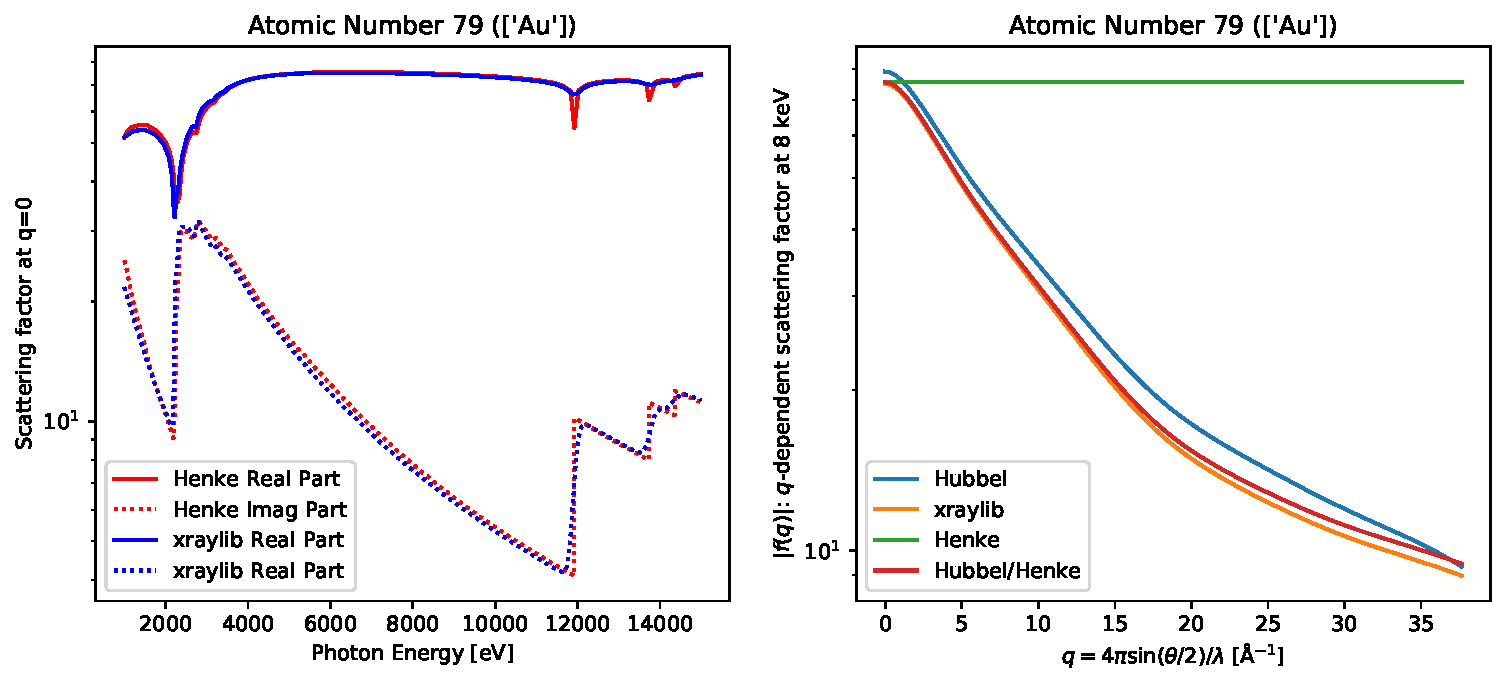
\includegraphics[width=\textwidth]{figures/formfactor_79.pdf} 
   \caption{Energy-dependent form factor in the forward scattering direction and the $Q$-dependent form factor.  Comparison between Henke tables and \texttt{xraylib} for gold.  The plots were generated with the file \texttt{developer/rkirian/misc/scattering\_factors.py}.}
   \label{fig:forms}
\end{figure} 


\section{bornagain}

These Henke scattering factors (at $q=0$) are returned as a single complex number $f$ from the function \texttt{get\_scattering\_factors(Z,E)}, which is in the \texttt{bornagain.simulate.atoms} sub-module.  \texttt{bornagain} also has wrappers to the xraylib functions for convenience since they use different units and they are not vectorized functions (hence they are very slow).  The combined Hubbel form factors and Henke dispersion corrections may be accessed through the function \texttt{bornagain.simulate.atoms.hubbel\_henke\_atomic\_form\_factors}.

%%%%%%%%%%%%%%%%%%%%%%%%%%%%%%%%%%%%%%%%%%%%%%%%%%%%%%%%%%%%%%%%%%%%%%%%%
\section{Getting to the density}
%%%%%%%%%%%%%%%%%%%%%%%%%%%%%%%%%%%%%%%%%%%%%%%%%%%%%%%%%%%%%%%%%%%%%%%%%

We are provided with $f(q)$ from the Hubbel tables, along with the relation 
\begin{align}
  \rho(r) &= \frac{1}{2 \pi^2} \int_0^\infty     [q f(q)]  \frac{\sin(qr)}{r}dq  \;. \label{eqn:trans}
\end{align}
Note that we should treat the case of $r\rightarrow 0$ with care since we have have $\sin(qr)/r \rightarrow q$ in that limit.  Thus we have a separate expression for $\rho(0)$:
\begin{align}
  \rho(0) &= \frac{1}{2 \pi^2} \int_0^\infty     [q^2 f(q)]  dq  \;. \label{eqn:trans0}
\end{align}
We aim to do this integral numerically.  We will discretize both $r$ and $q$ as follows:
\begin{align}
r_n &= n\Delta r \\
q_k &= k \Delta q
\end{align}
where $n$ and $k$ are integers.  The approximate integral is
\begin{align}
\rho(r_n) &\approx  \frac{1}{2 \pi^2 n\Delta r }\sum_{k=0}^{N-1}     [k \Delta q f(k \Delta q)]  \sin(k \Delta q n\Delta r) \Delta q \; .
\end{align}
We can do the above integral quickly if we use a Fast Fourier Transform (FFT) algorithm.  To see how this is done, firstly note that the sin transform above is just the imaginary part of the Fourier Transform.  With some foresight, we relate our gridpoints according to $\Delta q  = 2\pi / \Delta r N$, which gives us
\begin{align}
\rho(r_n) &\approx  \frac{1}{ \pi n\Delta r^2 }\text{Im}\left\{ \frac{1}{N}\sum_{k=0}^{N-1}     [k \Delta q f(k \Delta q)]  \exp\left(2\pi i \frac{ k  n}{N}\right) \right\} \; .
\end{align}
In numpy, the inverse FFT is defined in the following way:
\begin{align}\label{eqn:idft}
a_n = \text{FFT}^{-1}\left\{ A_k \right\}_n = \frac{1}{N}\sum_{k=0}^{N-1}A_k\exp\left(2\pi i \frac{nk}{N}\right) \qquad n = 0,\ldots,N-1
\end{align}
If we define
\begin{align}
F_k &= k \Delta q F(k \Delta q) 
\end{align}
we arrive at the desired expression
\begin{align}\label{eqn:rhor}
\rho(n \Delta r) &\approx \frac{1}{\pi n \Delta r^2 } \text{Im} \left\{ \frac{1}{N}  \sum_{k=0}^{N-1}    F_k  \exp\left( 2\pi i \frac{nk}{ N} \right) \right\} = \frac{1}{\pi n \Delta r^2 } \text{Im}\left\{ \text{FFT}^{-1}\left\{ F_k \right\}_n\right\} \; .
\end{align}
Equation \ref{eqn:rhor} has been tested and shown to agree in the case of the hydrogen atom, as shown in figure \ref{fig:hydrogen} (the example script \texttt{scattering\_factors.py} that generated this plot is found in bornagain).  However, there are some issues that remain at this time (1) the density near $r=0$ has a noticable error, and (2) there are oscillatory artifacts that might be due to the truncation of $f(q)$.

\begin{figure}[htbp]
   \centering
   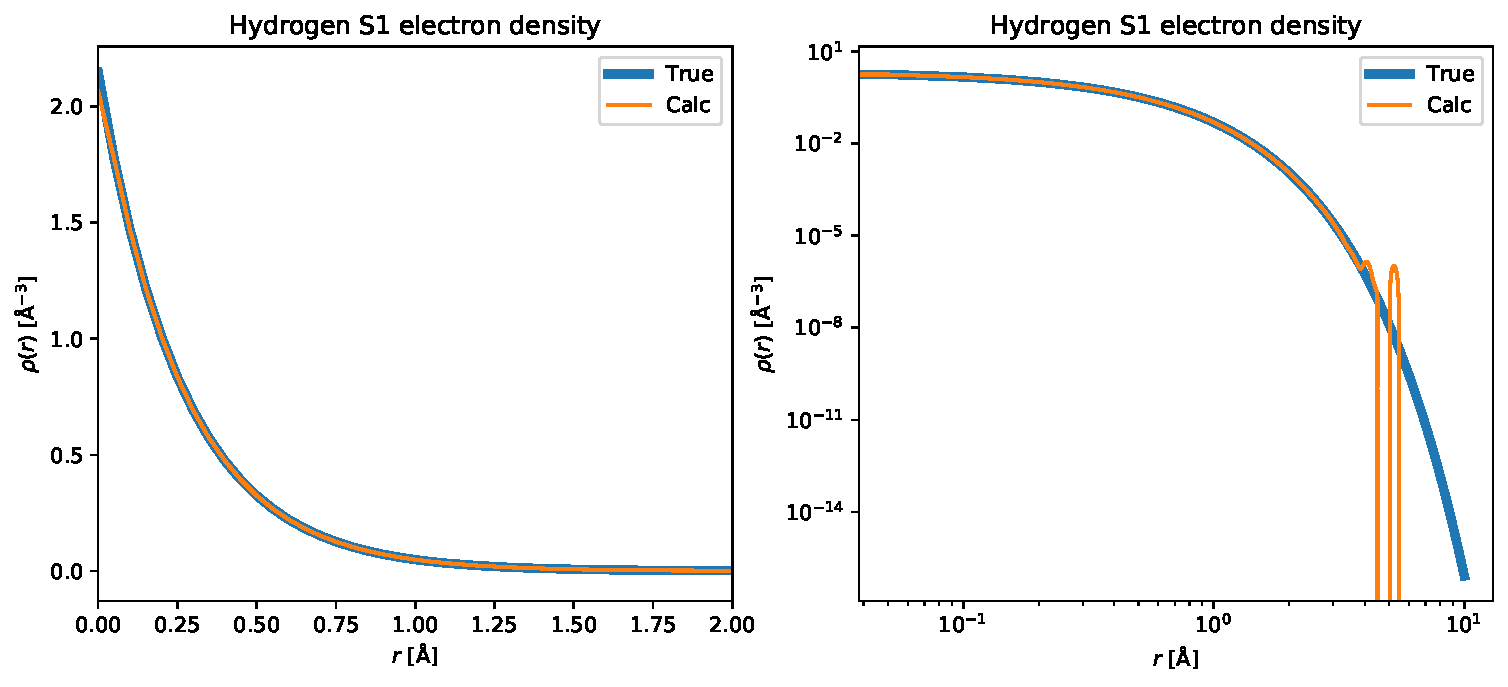
\includegraphics[width=\textwidth]{figures/hydrogen_density_1.pdf} 
   \caption{Hydrogen density calculated according to equation \ref{eqn:rhor}, compared against the analytic wavefunction $|\Psi(r)|^2=e^{-2 r/a_0}/\pi a_0^3$.}
   \label{fig:hydrogen}
\end{figure}

\section{Appendix}

\subsection{Fourier transform of rotationally symmetric object}
\label{sec:3d1d}

If we consider just a single atom situated at the origin, the atomic form factor is equal to
\begin{align}
 f(\vec{q})  = \int \rho(r) \exp(-i \vec{q}\cdot\vec{r}) \; d^3r \; .
\end{align}
Due to rotational symmetry, we are free to choose a convenient direction $\vec{q} = q \hvec{z}$ such that in the spherical coordinate system we have $\vec{q}\cdot\vec{r} =  q r \cos\theta$.  Now we write down our Fourier transform with reference only to the magnitudes $q$ and $r$:
\begin{align}
f(\vec{q})  &= \int_0^{2\pi} d\phi \int_0^\infty \rho(r) r^2 dr \int_0^\pi \sin\theta d\theta  \exp(-i q r \cos\theta)  \\
&=2\pi \int_0^\infty \rho(r) r^2 dr \int_{-1}^1  d\cos\theta  \exp(-i q r \cos\theta)  \\
&=2\pi \int_0^\infty \rho(r) r^2 dr \frac{1}{-iqr}\int_{iqr}^{-iqr}  du  \exp(u)  \\
&=2\pi \int_0^\infty \rho(r) r^2 dr \frac{\exp(iqr) - \exp(-iqr)}{iqr}   \\
f(q) &= \int_0^\infty \rho(r)   \frac{\sin(qr)}{qr}  4\pi r^2 dr  
\end{align}


\newpage




\bibliography{\jobname}
\bibliographystyle{plain}

\end{document}
